%  !TeX  root  =  user_guide.tex

\chapter{Обзор возможностей}\label{feature_glance}

% when the revision of a section has been finalized,
% comment out the following line:
%\updatedisclaimer

В разделе~\ref{label_getstarted} вы познакомились с QGIS и научились
некоторым простейшим операциям. В этой главе приводится более детальный обзор
возможностей QGIS. Большая часть функций будут объяснены и
описаны в руководстве позднее, в соответствующих разделах.

\section{Запуск и выход из QGIS}\label{label_startinqgis}

В разделе~\ref{samplesession} вы узнали, как запустить QGIS. Здесь же мы разберём
дополнительные параметры командной строки и варианты запуска.

\begin{itemize}
\item \nix{Предполагая, что QGIS установлен в каталог, указанный в PATH,
вы можете запустить QGIS, набрав в командной строке: \usertext{qgis} или
двойным нажатием на ссылке (или ярлыке) QGIS на Рабочем столе или в меню
Приложения.}
\item \win{Запустите QGIS через меню Пуск или через ярлык на Рабочем
столе или дважды нажав на значке файла проекта QGIS.}
\item \osx{Дважды нажмите значок в вашей папке Приложения. Если необходимо
запустить QGIS в оболочке, выполните
\usertext{/path-to-installation-executable/Contents/MacOS/Qgis}.}
\end{itemize}

Для выхода из QGIS, нажмите меню \{\nix{}\win{Файл} \osx{QGIS}\} \arrow
Выход,или используйте комбинацию клавиш \keystroke{Ctrl+Q}.

\subsection{Параметры командной строки}\index{параметры командной строки}
\label{label_commandline}

\nix При запуске \qg из командной строки можно указать дополнительные параметры.
Для получения полного списка параметров, введите в командной строке
\usertext{qgis ---help}. Описание параметров выглядит следующим образом:

\small
\begin{verbatim}
qgis --help
Quantum GIS - 1.5.0-Tethys 'Tethys' (exported)
Quantum GIS (QGIS) is a viewer for spatial data sets, including
raster and vector data.
Usage: qgis [options] [FILES]
  options:
        [--snapshot filename]           emit snapshot of loaded datasets to given file
        [--width width]                 width of snapshot to emit
        [--height height]               height of snapshot to emit
        [--lang language]               use language for interface text
        [--project projectfile]         load the given QGIS project
        [--extent xmin,ymin,xmax,ymax]  set initial map extent
        [--nologo]                      hide splash screen
        [--help]                        this text

  FILES:
    Files specified on the command line can include rasters,
    vectors, and QGIS project files (.qgs):
     1. Rasters - Supported formats include GeoTiff, DEM
        and others supported by GDAL
     2. Vectors - Supported formats include ESRI Shapefiles
        and others supported by OGR and PostgreSQL layers using
        the PostGIS extension
\end{verbatim}
\normalsize

\begin{Tip} \caption{\textsc{Пример использования параметров командной строки}}
Можно запускать QGIS, указав в командной строке один или несколько файлов
данных. Например, если вы находитесь в каталоге qgis\_sample\_data,
можно запустить QGIS с загрузкой векторного и растрового
слоёв следующим образом: \\
\usertext{qgis ./raster/landcover.img ./gml/lakes.gml}
\end{Tip}

\minisec{Параметр \usertext{---snapshot}}
Этот параметр позволяет создавать снимок текущего вида в формате PNG. Данная
функция применяется при большом количестве проектов и при необходимости
создания снимков имеющихся данных.

По умолчанию создаётся PNG-файл разрешением 800x600 пикселей. Разрешение
можно изменить посредством параметров
\usertext{---width} и \usertext{---height}. Имя файла указывается после параметра
\usertext{---snapshot}.

\minisec{Параметр \usertext{---lang}}
Основываясь на языковых настройках операционной системы, QGIS выбирает
соответствующий язык интерфейса пользователя (локализацию). Если вы хотите
сменить локализацию интерфейса, этот параметр позволяет задать языковой код. Например:
\usertext{---lang=it} запускает QGIS с итальянской локализацией. Список
поддерживаемых в настоящее время языков с их кодами и состоянием перевода можно
уточнить на веб-странице
\url{http://www.qgis.org/wiki/GUI_Translation_Progress}

\minisec{Параметр \usertext{---project}}
При запуске QGIS можно открыть существующий файл проекта. Просто
добавьте параметр \usertext{---project} и укажите файл проекта. QGIS
запустится со всеми слоями, указанными в данном файле проекта.

\minisec{Параметр \usertext{---extent}}
Используйте этот параметр для запуска с определенным охватом карты.
Необходимо добавить прямоугольник охвата, в следующем порядке (значения
разделяются запятой):
\begin{verbatim}
--extent xmin,ymin,xmax,ymax
\end{verbatim}

\minisec{параметр \usertext{---nologo}}
Этот параметр командной строки скрывает окно приветствия при запуске QGIS.

\section{Интерфейс QGIS}\index{интерфейс}
\label{label_qgismainwindow}

В приложении \qg, графический интерфейс пользователя разделяется на шесть основных
областей, которые перечислены ниже и отмечены соответствующими номерами на рисунке.

\begin{figure}[ht]
   \centering
    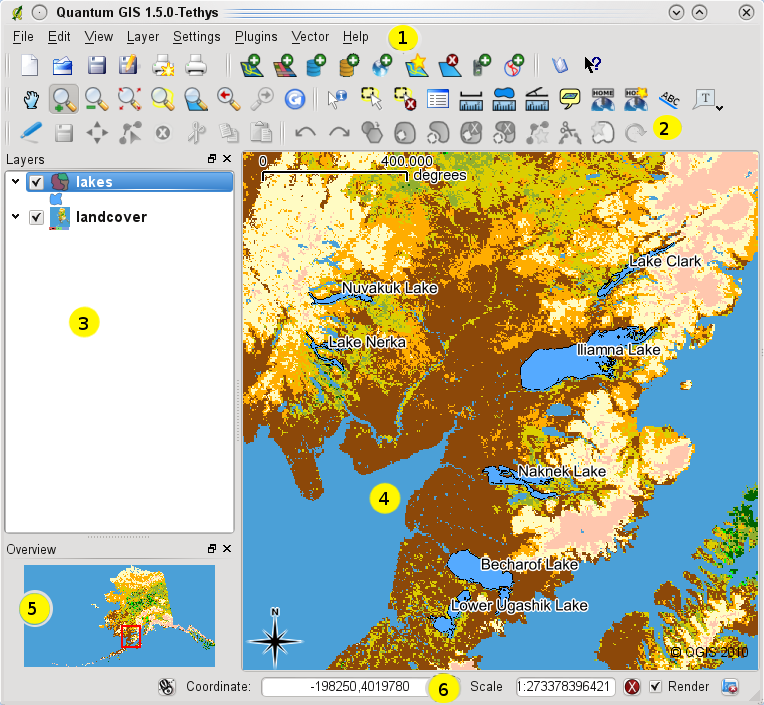
\includegraphics[clip=true, width=12cm]{startup}
    \caption{Интерфейс QGIS с открытым примером данных Alaska \wincaption} \label{fig:startup}
\end{figure}

\textbf{Примечание:} Внешний вид элементов интерфейса (заголовки
и т.\,п.) может отличаться, в зависисмости от операционной системы и
менеджера окон.\\

Интерфейс QGIS разделяется на шесть областей:

\begin{tabular}{p{5cm} p{5cm}}
%\centering
1. Главное меню & 4. Область карты \\
2. Панель инструментов & 5. Обзорная карта \\
3. Легенда & 6. Строка состояния \\
\end{tabular}

Компоненты интерфейса QGIS, комбинации клавиш и контекстная справка более
подробно описаны в следующих разделах.
% \newpage

\subsection{Главное меню}\label{label_menubar}
\index{меню}

Главное меню предоставляет доступ ко всем возможностям QGIS в виде
стандартного иерархического меню. Ниже показаны меню верхнего уровня
и краткое описание их содержимого, а также значки соответствующих им
инструментов по мере их появления на панели инструментов и комбинации
клавиш клавиатуры.\footnote{Комбинации клавиш могут быть настроены вручную (пункт
<<Комбинации клавиш>> в меню <<Установки>>), приведённые комбинации используются
по умолчанию.}
Несмотря на то, что большинству пунктов меню соответствует свой инструмент,
и наоборот, меню и панели инструментов организованы по-разному.
Панель инструментов, в которой находится инструмент, показана после каждого
пункта меню в виде флажка. Дополнительную информацию об инструментах
и панелях инструментов можно найти в Разделе~\ref{label_toolbars}.

\begin{tabbing}
\hspace{5.5cm}\=\hspace{3cm}\=\hspace{3.5cm}\= \kill
\hspace{1cm} Пункт меню \> Комбинация клавиш \> Справка \> Панель инструментов\\
\end{tabbing}

\begin{itemize}
\item \mainmenuopt{Файл}
\begin{tabbing}
\hspace{4.5cm}\=\hspace{3cm}\=\hspace{3.5cm}\= \kill
\dropmenuopttwo{mActionFileNew}{Новый проект}
        \> \keystroke{Ctrl+N}
        \> см. Раздел \ref{sec:projects}
        \> \dropmenucheck{Файл} \\
\dropmenuopttwo{mActionFileOpen}{Открыть проект}
        \> \keystroke{Ctrl+O}
        \> см. Раздел \ref{sec:projects}
        \> \dropmenucheck{Файл} \\
\dropmenuopt{Открыть недавние проекты}
        \>
        \> см. Раздел \ref{sec:projects} \\
\dropmenuopttwo{mActionFileSave}{Сохранить проект}
        \> \keystroke{Ctrl+S}
        \> см. Раздел \ref{sec:projects}
        \> \dropmenucheck{Файл} \\
\dropmenuopttwo{mActionFileSaveAs}{Сохранить проект как\ldots}
        \> \keystroke{Ctrl+Shift+S}
  \> см. Раздел \ref{sec:projects}
        \> \dropmenucheck{Файл} \\
\dropmenuopttwo{mActionSaveMapAsImage}{Сохранить как изображение}
        \>
        \> см. Раздел \ref{sec:output} \\
\dropmenuopttwo{mActionNewComposer}{Создать компоновку карты}
        \> \keystroke{Ctrl+P}
        \> см. Раздел \ref{label_printcomposer}
        \> \dropmenucheck{Файл} \\
\dropmenuopttwo{mActionComposerManager}{Управление компоновками}
        \>
        \> см. Раздел \ref{label_printcomposer}
        \> \dropmenucheck{Файл} \\
\dropmenuopt{Компоновки карт}
        \>
        \> см. Раздел \ref{label_printcomposer} \\
\dropmenuopttwo{mActionFileExit}{Выход}
        \> \keystroke{Ctrl+Q} \\
\end{tabbing}

\item \mainmenuopt{Правка}
\begin{tabbing}
\hspace{6.5cm}\=\hspace{3cm}\=\hspace{3.5cm}\= \kill
\dropmenuopttwo{mActionUndo}{Отменить}
        \> \keystroke{Ctrl+Z}
        \> см. Раздел \ref{sec:advanced_edit}
        \> \dropmenucheck{Дополнительные функции оцифровки} \\
\dropmenuopttwo{mActionRedo}{Вернуть}
        \> \keystroke{Ctrl+Shift+Z}
        \> см. Раздел \ref{sec:advanced_edit}
        \> \dropmenucheck{Дополнительные функции оцифровки} \\
\dropmenuopttwo{mActionEditCut}{Вырезать объекты}
        \> \keystroke{Ctrl+X}
        \> см. Раздел \ref{sec:edit_existing_layer}
        \> \dropmenucheck{Оцифровка} \\
\dropmenuopttwo{mActionEditCopy}{Копировать объекты}
        \> \keystroke{Ctrl+C}
        \> см. Раздел \ref{sec:edit_existing_layer}
        \> \dropmenucheck{Оцифровка} \\
\dropmenuopttwo{mActionEditPaste}{Вставить объекты}
        \> \keystroke{Ctrl+V}
        \> см. Раздел \ref{sec:edit_existing_layer}
        \> \dropmenucheck{Оцифровка} \\
\dropmenuopttwo{mActionEditPaste}{Переместить объект}
        \>
        \> см. Раздел \ref{sec:edit_existing_layer}
        \> \dropmenucheck{Оцифровка} \\
\dropmenuopttwo{mActionDeleteSelected}{Удалить выделенное}
        \>
        \> см. Раздел \ref{sec:edit_existing_layer}
        \> \dropmenucheck{Оцифровка} \\
\dropmenuopttwo{mActionSimplify}{Упростить объект}
        \>
        \> см. Раздел \ref{sec:advanced_edit}
        \> \dropmenucheck{Дополнительные функции оцифровки} \\
\dropmenuopttwo{mActionAddRing}{Добавить кольцо}
        \>
        \> см. Раздел \ref{sec:advanced_edit}
        \> \dropmenucheck{Дополнительные функции оцифровки} \\
\dropmenuopttwo{mActionAddIsland}{Добавить часть}
        \>
        \> см. Раздел \ref{sec:advanced_edit}
        \> \dropmenucheck{Дополнительные функции оцифровки} \\
\dropmenuopttwo{mActionDeleteRing}{Удалить кольцо}
        \>
        \> см. Раздел \ref{sec:advanced_edit}
        \> \dropmenucheck{Дополнительные функции оцифровки} \\
\dropmenuopttwo{mActionDeletePart}{Удалить часть}
        \>
        \> см. Раздел \ref{sec:advanced_edit}
        \> \dropmenucheck{Дополнительные функции оцифровки} \\
\dropmenuopttwo{mActionReshape}{Корректировать объекты}
        \>
        \> см. Раздел \ref{sec:advanced_edit}
        \> \dropmenucheck{Дополнительные функции оцифровки} \\
\dropmenuopttwo{mActionSplitFeatures}{Разбить объекты}
        \>
        \> см. Раздел \ref{sec:advanced_edit}
        \> \dropmenucheck{Дополнительные функции оцифровки} \\
\dropmenuopttwo{mActionMergeFeatures}{Объединить выбранные объекты}
        \>
        \> см. Раздел \ref{sec:advanced_edit}
        \> \dropmenucheck{Дополнительные функции оцифровки} \\
\dropmenuopttwo{mActionNodeTool}{Редактирование узлов}
        \>
        \> см. Раздел \ref{sec:edit_existing_layer}
        \> \dropmenucheck{Оцифровка} \\
\dropmenuopttwo{mActionRotatePointSymbols}{Повернуть значки}
        \>
        \> см. Раздел \ref{sec:advanced_edit}
        \> \dropmenucheck{Дополнительные функции оцифровки} \\
\end{tabbing}

После активации \toolbtntwo{mActionToggleEditing}{Режима редактирования}
для слоя, в меню \mainmenuopt{Правка} появится значок создания объекта,
в зависимости от типа слоя (точечный, линейный или полигональный). \\

\begin{tabbing}
\hspace{6.5cm}\=\hspace{3cm}\=\hspace{3.5cm}\= \kill
\dropmenuopttwo{mActionCapturePoint}{Создать точку}
        \>
        \> см. Раздел \ref{sec:edit_existing_layer}
        \> \dropmenucheck{Оцифровка} \\
\dropmenuopttwo{mActionCaptureLine}{Создать линию}
        \>
        \> см. Раздел \ref{sec:edit_existing_layer}
        \> \dropmenucheck{Оцифровка} \\
\dropmenuopttwo{mActionCapturePolygon}{Создать полигон}
        \>
        \> см. Раздел \ref{sec:edit_existing_layer}
        \> \dropmenucheck{Оцифровка} \\
\end{tabbing}


\item \mainmenuopt{Вид}
\begin{tabbing}
\hspace{6.5cm}\=\hspace{3cm}\=\hspace{3.5cm}\= \kill
\dropmenuopttwo{mActionPan}{Прокрутка карты}
        \>
        \> \> \dropmenucheck{Навигация} \\
\dropmenuopttwo{mActionZoomIn}{Увеличить}
        \> \keystroke{Ctrl+\textbf{+}}
        \> \> \dropmenucheck{Навигация} \\
\dropmenuopttwo{mActionZoomOut}{Уменьшить}
        \> \keystroke{Ctrl+\textbf{-}}
        \> \> \dropmenucheck{Навигация} \\
\dropmenuopttwo{mActionSelect}{Выбрать объекты}
        \>
        \> \> \dropmenucheck{Атрибуты} \\
\dropmenuopttwo{mActionDeselectAll}{Снять выделение во всех слоях}
        \>
        \> \> \dropmenucheck{Атрибуты} \\
\dropmenuopttwo{mActionIdentify}{Определить объекты}
        \> \keystroke{Ctrl-Alt-I}
        \> \> \dropmenucheck{Атрибуты} \\
\dropmenuopttwo{mActionMeasure}{Измерить линию}
        \> \keystroke{Ctrl-Alt-M}
        \> \> \dropmenucheck{Атрибуты} \\
\dropmenuopttwo{mActionMeasureArea}{Измерить площадь}
        \> \keystroke{Ctrl-Alt-J}
        \> \> \dropmenucheck{Атрибуты} \\
\dropmenuopttwo{mActionMeasureAngle}{Измерить угол}
        \>
        \> \> \dropmenucheck{Атрибуты} \\
\dropmenuopttwo{mActionOpenTable}{Полный охват}
        \> \keystroke{Ctrl-Alt-F}
        \> \> \dropmenucheck{Навигация} \\
\dropmenuopttwo{mActionZoomToLayer}{Увеличить до слоя}
        \>
        \> \> \dropmenucheck{Навигация} \\
\dropmenuopttwo{mActionZoomToSelected}{Увеличить до выделенного}
        \> \keystroke{Ctrl+J}
        \> \> \dropmenucheck{Навигация} \\
\dropmenuopttwo{mActionZoomLast}{Предыдущий охват}
        \>
        \> \> \dropmenucheck{Навигация} \\
\dropmenuopttwo{mActionZoomNext}{Следующий охват}
        \>
        \> \> \dropmenucheck{Навигация} \\
\mainmenuopt{Фактический размер}
        \>
        \> \>  \\
\dropmenuopttwo{mActionMapTips}{Всплывающие описания}
        \>
        \> \> \dropmenucheck{Атрибуты} \\
\dropmenuopttwo{mActionNewBookmark}{Новая закладка}
        \> \keystroke{Ctrl+B}
        \> см. Раздел \ref{sec:bookmarks}
\> \dropmenucheck{Атрибуты} \\
\dropmenuopttwo{mActionShowBookmarks}{Показать закладки}
        \> \keystroke{Ctrl-Alt-B}
        \> см. Раздел \ref{sec:bookmarks}
        \> \dropmenucheck{Атрибуты} \\
\dropmenuopttwo{mActionDraw}{Обновить}
        \> \keystroke{Ctrl+R}
        \> \> \dropmenucheck{Навигация} \\
\mainmenuopt{Уровень детализации}
        \>
        \> см. Раздел \ref{sec:tilesets}
        \> \dropmenucheck{Уровень детализации} \\
\mainmenuopt{GPS-слежение}
        \>
        \> см. Раздел \ref{sec:gpstracking}
        \> \dropmenucheck{GPS слежение} \\
\end{tabbing}

\item \mainmenuopt{Слой}
\begin{tabbing}
\hspace{6.5cm}\=\hspace{3cm}\=\hspace{3.5cm}\= \kill
\dropmenuopt{Создать}
        \>
        \> см. Раздел \ref{sec:create shape}
        \> \dropmenucheck{Управление слоями} \\
\dropmenuopttwo{mActionAddNonDbLayer}{Добавить векторный слой}
        \> \keystroke{Ctrl+Shift+V}
        \>
        см. Раздел \ref{label_workingvector}
        \> \dropmenucheck{Управление слоями} \\
\dropmenuopttwo{mActionAddRasterLayer}{Добавить растровый слой}
        \> \keystroke{Ctrl+Shift+R}
        \>
        см. Раздел \ref{label_raster}
        \> \dropmenucheck{Управление слоями} \\
\dropmenuopttwo{mActionAddLayer}{Добавить слой PostGIS}
        \> \keystroke{Ctrl+Shift+D}
        \>
        см. Раздел \ref{label_postgis}
        \> \dropmenucheck{Управление слоями} \\
\dropmenuopttwo{mActionAddSpatiaLiteLayer}{Добавить слой SpatiaLite}
        \> \keystroke{Ctrl+Shift+L}
        \>
        см. Раздел \ref{label_spatialite}
        \> \dropmenucheck{Управление слоями} \\
\dropmenuopttwo{mActionAddWmsLayer}{Добавить WMS-слой}
        \> \keystroke{Ctrl+Shift+W}
        \>
        см. Раздел \ref{sec:ogc-wms}
        \> \dropmenucheck{Управление слоями} \\
\dropmenuopttwo{mActionOpenTable}{Открыть таблицу атрибутов}
        \> \>
        \> \dropmenucheck{Атрибуты} \\
\dropmenuopttwo{mActionFileSave}{Сохранить изменения}
        \> \>
        \> \dropmenucheck{Оцифровка} \\
\dropmenuopttwo{mActionToggleEditing}{Режим редактирования}
        \> \>
        \> \dropmenucheck{Оцифровка} \\
\mainmenuopt{Сохранить как\ldots}
        \\
\mainmenuopt{Сохранить выделение как\ldots}
        \\
\dropmenuopttwo{mActionRemoveLayer}{Удалить слой}
        \> \keystroke{Ctrl+D}
        \>
        \> \dropmenucheck{Управление слоями} \\
\mainmenuopt{Свойства}
        \\
\mainmenuopt{Запрос\ldots}
        \\
\dropmenuopttwo{mActionInOverview}{Добавить в обзор}
        \> \keystroke{Ctrl+Shift+O}
        \\
\dropmenuopttwo{mActionAddAllToOverview}{Добавить все в обзор}
        \\
\dropmenuopttwo{mActionRemoveAllFromOverview}{Удалить все из обзора}
        \\
\dropmenuopttwo{mActionHideAllLayers}{Скрыть все слои}
        \> \keystroke{Ctrl+Shift+H}
        \\
\dropmenuopttwo{mActionShowAllLayers}{Показать все слои}
        \> \keystroke{Ctrl+Shift+U}
        \\
\dropmenuopttwo{labeling}{Подписи}
        \> \>
        \> \dropmenucheck{Атрибуты} \\
\end{tabbing}

\item \mainmenuopt{Установки}
\begin{tabbing}
\hspace{6.5cm}\=\hspace{3cm}\=\hspace{3.5cm}\= \kill
\dropmenuopt{Панели}
        \>
        \>
        \\
\dropmenuopt{Панели инструментов}
        \>
        \>
        \\
\mainmenuopt{Полноэкранный режим}
        \>\keystroke{Ctrl-F}
        \>
        \\
\dropmenuopttwo{mActionProjectProperties}{Свойства проекта}
        \> \keystroke{Ctrl-Alt-P}
        \> см. Раздел \ref{sec:projects} \\
\dropmenuopttwo{mActionCustomProjection}{Ввод системы координат}
        \> \> см. Раздел \ref{sec:customprojections} \\
\mainmenuopt{Управление стилями}
        \> \> \\
\dropmenuopttwo{mActionOptions}{Комбинации клавиш}
        \> \> \\
\dropmenuopttwo{mActionOptions}{Параметры}
        \> \> см. Раздел \ref{subsec:gui_options} \\
\end{tabbing}

\item \mainmenuopt{Модули} "--- (Следующие пункты меню добавляются
подключаемыми модулями после их загрузки.)
\begin{tabbing}
\hspace{6.5cm}\=\hspace{3cm}\=\hspace{3.5cm}\= \kill
\dropmenuopttwo{mActionShowPluginManager}{Управление модулями}
        \> \> см. Раздел \ref{sec:managing_plugins} \dropmenucheck{Модули}
        \\
        \mainmenuopt{Консоль Python}
        \> \>
        \\
\end{tabbing}

\item \mainmenuopt{Справка}
\begin{tabbing}
\hspace{6.5cm}\=\hspace{3cm}\=\hspace{3.5cm}\= \kill
\dropmenuopttwo{mActionHelpContents}{Содержание}
        \> \keystroke{F1}
        \>
        \> \dropmenucheck{Справка}\\
\dropmenuopttwo{mActionQgisHomePage}{Веб-сайт QGIS}
        \> \keystroke{Ctrl+H}
        \>
        \\
\dropmenuopttwo{mActionCheckQgisVersion}{Проверить версию QGIS}
        \\
\dropmenuopttwo{mActionHelpAbout}{О программе}
        \\
\end{tabbing}

\end{itemize}

\textbf{Примечание:} \nix Пункты главного меню, перечисленные выше,
являются стандартными в графической среде KDE. В графической среде GNOME
меню <<Установки>> отсутствует, а его пункты расположены следующим образом:
\begin{tabbing}
\dropmenuopttwo{mActionProjectProperties}{Свойства проекта} \hspace{3cm}\=
\dropmenucheck{Файл} \\
\dropmenuopttwo{mActionOptions}{Параметры} \hspace{3cm}\>
\dropmenucheck{Правка}\\
\dropmenuopttwo{mActionOptions}{Комбинации клавиш} \hspace{3cm}\>
\dropmenucheck{Правка}\\
\mainmenuopt{Управление стилями} \hspace{3cm}\>
\dropmenucheck{Правка}\\
\dropmenuopttwo{mActionCustomProjection}{Ввод системы координат}\hspace{3cm}\>
\dropmenucheck{Правка} \\
\dropmenuopt{Панели} \hspace{3cm}\>
\dropmenucheck{Вид} \\
\dropmenuopt{Панели инструментов} \hspace{3cm}\>
\dropmenucheck{Вид} \\
\mainmenuopt{Полноэкранный режим} \hspace{3cm}\>
\dropmenucheck{Вид} \\
\mainmenuopt{Уровень детализации} \hspace{3cm}\>
\dropmenucheck{Вид} \\
\mainmenuopt{GPS-слежение} \hspace{3cm}\>
\dropmenucheck{Вид} \\
\end{tabbing}

%See Appendix \ref{app_menu} for complete descriptions of the menu items.

\subsection{Панели инструментов}\label{label_toolbars}
\index{панели инструментов}

Панели инструментов обеспечивают доступ к большинству тех же функций,
что и меню, а также содержат дополнительные инструменты для работы с
картой. Для каждого пункта панели инструментов также доступна всплывающая
подсказка (для её получения просто задержите мышь над пунктом панели инструментов).

Каждую панель инструментов можно перемещать в зависимости от ваших
потребностей. Кроме того, каждую панель инструментов можно скрыть при
помощи контекстного меню, которое вызывается щелчком правой кнопкой мыши
на соответствующей панели.

\begin{Tip}
\caption{\textsc{Восстановление панелей инструментов}} \index{внешний вид!панели инструментов}
Если вы случайно скрыли все панели инструментов, можно вернуть их обратно,
используя пункт меню \mainmenuopt{Вид} \arrow \dropmenuopt{Панели инструментов}.
\end{Tip}

\subsection{Легенда}\label{label_legend}
\index{легенда}

Область легенды предназначена для установки видимости и порядка
расположения слоев карты. Порядок расположения слоев означает, что слои
находящиеся ближе к верхней части легенды, отрисовываются в окне карты
над слоями, перечисленными в легенде ниже. Флажок у каждого элемента
легенды используется для показа или сокрытия слоя.\index{слой!видимость}

Слои можно объединять в группы. Для этого поместите курсор мыши в окне
легенды карты, щёлкните правой кнопкой мыши и выберите пункт
\dropmenuopt{Добавить группу}. В легенде появится новая группа (папка).
Теперь перетащите слои на значок папки.

Группы дают возможность переключать видимость всех слоев в группе одним действием.
Для вывода слоев из группы щёлкните правой кнопкой мыши на значке слоя и выберите
пункт \dropmenuopt{Сделать элементом первого уровня}. Чтобы переименовать
папку, выберите \dropmenuopt{Переименовать}, щёлкнув правой кнопкой мыши на
имени группы.

Содержание контекстного меню, доступного при нажатии правой кнопки мыши
на слое, зависит от того, на каком слое в окне легенды вы нажали правой
кнопкой"--- растровом или векторном. Для векторных слоев GRASS
\dropmenuopt{Режим редактирования} недоступен. Редактированию векторных
слоев GRASS рассматривается в разделе~\ref{grass_digitising}.

\begin{itemize}

\item \textbf{Контекстное меню для растровых слоев}
\begin{itemize}
\item \dropmenuopt{Увеличить до границ слоя}
\item \dropmenuopt{Увеличить до наилучшего масштаба (100\%)}
\item \dropmenuopt{Показать в обзоре}
\item \dropmenuopt{Удалить}
\item \dropmenuopt{Свойства}
\item \dropmenuopt{Переименовать}
\item \dropmenuopt{Добавить группу}
\item \dropmenuopt{Развернуть все}
\item \dropmenuopt{Свернуть все}
%%\item \dropmenuopt{Show file groups}
\end{itemize}

\item \textbf{Контекстное меню для векторных слоев}
\begin{itemize}
\item \dropmenuopt{Увеличить до границ слоя}
\item \dropmenuopt{Показать в обзоре}
\item \dropmenuopt{Удалить}
\item \dropmenuopt{Открыть таблицу атрибутов}
\item \dropmenuopt{Режим редактирования (недоступен для слоев GRASS)}
\item \dropmenuopt{Сохранить как\ldots}
\item \dropmenuopt{Сохранить выделение как\ldots}
\item \dropmenuopt{Запрос}
\item \dropmenuopt{Свойства}
%% \item \dropmenuopt{Make to toplevel item}
\item \dropmenuopt{Переименовать}
\item \dropmenuopt{Добавить группу}
\item \dropmenuopt{Развернуть все}
\item \dropmenuopt{Свернуть все}
%%\item \dropmenuopt{Show file groups}
\end{itemize}

\item \textbf{Контекстное меню для групп слоев}
\begin{itemize}
\item \dropmenuopt{Удалить}
\item \dropmenuopt{Переименовать}
\item \dropmenuopt{Добавить группу}
\item \dropmenuopt{Развернуть все}
\item \dropmenuopt{Свернуть все}
%%\item \dropmenuopt{Show file groups}
\end{itemize}

\end{itemize}

В случае, если несколько источников векторных данных имеют одинаковый
тип вектора и те же атрибуты, их символика может быть сгруппирована.
Это означает, что если символика одного источника данных изменится,
другие автоматически получат новую символику. Для группировки символики,
вызовите контекстное меню в окне легенды и выберите
\dropmenuopt{Добавить группу}. В результате будет создана новая группа слоёв
и станет возможным перетаскивание файла из одной группы в другую. Если это будет
сделано, символика будет сгруппирована. Обратите внимание, что QGIS
позволяет перетаскивание, только если два слоя имеют возможность
обмениваться символикой (тот же тип векторной геометрии и те же атрибуты).

%% isn't included in Titan anymore, except for an "toggle overview"
%Each legend entry can show the following mini icons:
%
%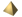
\includegraphics[width=0.7cm]{pyramid} This is a raster
%that has pyramids built for it to improve rendering efficiency (see
%Section \ref{raster_pyramids}).\\
%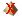
\includegraphics[width=0.7cm]{no_pyramid} This is a
%raster that has no pyramid layers (see Section \ref{raster_pyramids}).\\
%
\includegraphics[width=0.7cm]{inoverview} This layer is
%shown in the overview map area as well as in the main map window.\\
%
\includegraphics[width=0.7cm]{editable} This is a vector
%layer that is currently enabled for editing.\\

\subsection{Область карты}\label{label_mapview}
\index{карта!область}

Это наиболее важная часть QGIS"--- в этой области отображаются карты. Карта,
отображаемая в области, зависит от того, какие векторные и растровые
слои загружены в QGIS (см. соответствующие разделы). Данные в окне карты
можно панорамировать (прокручивать, смещать фокус отображения карты на
другую область) и масштабировать (увеличивать или уменьшать). Также с
картой можно выполнять многие другие операции, которые перечислены выше
в описаниях меню и панелей инструментов. Область карты и легенда тесно
связаны друг с другом"--- карта отображает изменения, вносимые в легенде.

\begin{Tip}\caption{\textsc{Масштабирование карты с помощью колеса мыши}}\index{масштабирование!колесо мыши}
Для увеличения и уменьшения масштаба карты можно пользоваться колесом мыши.
Поместите курсор мыши внутри области карты и вращайте колесо вперед (от себя)
для увеличения масштаба (приближения) и назад для уменьшения масштаба
(удаления). Масштабирование производится относительно центра, которым
является положение курсора мыши. Поведение колеса мыши при масштабировании,
можно настроить по своему вкусу на вкладке \tab{Инструменты} в
меню \mainmenuopt{Установки} \arrow \dropmenuopt{Праметры}.
\end{Tip}

\begin{Tip}\caption{\textsc{Панорамирование карты, используя клавиши
со стрелками и клавишу пробела}}\index{панорамирование!клавиши управления курсором}
Для панорамирования (прокрутки) карты можно пользоваться клавишами со стрелками.
Поместите курсор мыши внутри области карты, нажмите клавишу вправо
для панорамирования на восток, влево"--- для панорамирования
на запад, вверх"--- для панорамирования на север и вниз"--- для
панорамирования на юг. Также можно панорамировать карту используя клавишу
пробел: просто передвигайте курсор, удерживая нажатой клавишу <<пробел>>.
\end{Tip}

\subsection{Обзорная карта}\label{label_mapoverview}
\index{карта!обзорная}

Панель Обзора (или обзорная карта) предоставляет вид полного охвата слоев,
добавленных в обзор. Панель обзора можно включить в меню
\mainmenuopt{Вид} \arrow \dropmenuopt{Панели}. Внутри окна обзора
находится прямоугольник, который показывает текущий охват карты. Это позволяет
быстро определять, какая часть карты сейчас просматривается в QGIS. Обратите
внимание, что подписи в окне обзора не отображаются, даже если они включены для
соответствующих слоёв.

Добавить в Обзор единичный слой можно, щёлкнув правой кнопкой мыши на этом
слое в легенде и выбрав \checkbox{Показать в обзоре}. Также можно
добавлять и удалять слои из обзорной карты, используя соответствующие
пункты в меню Слой.

Если нажать и переместить красный прямоугольник, показывающий текущий охват
в обзорной карте, область карты обновится соответствующим образом.

\subsection{Строка состояния}\label{label_statusbar}

Строка состояния отображает текущую позицию в координатах карты (например,
в метрах или десятичных градусах) курсора мыши при его перемещении в окне
карты. Слева от отображаемых координат в строке состояния, находится
маленькая кнопка, которая позволяет переключаться между отображением
координат позиции курсора и координат границ вывода карты при
масштабировании и панорамировании.

Индикатор выполнения в строке состояния, отображает процесс отрисовки
(рендеринга) каждого слоя в окне карты. В некоторых случаях, таких, как
подсчёт статистики в растровых слоях, индикатор состояния используется
для отображения статуса длительных операций.

В случае, если будет доступен новый модуль или обновление для
существующего модуля, в строке состояния появится новое сообщение. Справа
в строке состояния, находится маленький флажок, который используется для
временного прекращения отрисовки слоев в окне карты
(см. Раздел~\ref{subsec:redraw_events} ниже). Последним справа в строке
состояния находится значок Преобразования координат. Нажатие на нем
открывает диалоговое окно Системы координат текущего проекта.

\begin{Tip}\caption{\textsc{Вычисление правильного масштаба карты}}\index{масштаб!вычисление}
При запуске QGIS, единицами измерения по умолчанию являются градусы, и предполагается,
что любые координаты в ваших слоях также заданы в градусах. Для
получения правильных значений масштаба, можно вручную изменить единицы
слоя на метры на вкладке \tab{Общие} пункта меню \mainmenuopt{Установки}
\arrow \dropmenuopt{Свойства проекта}, либо выбрать систему
координат (CRS) нажатием на значке
\toolbtntwo{mIconProjectionDisabled}{Преобразование координат} в правом
нижнем углу строки состояния. В последнем случае, единицы слоя
будут установлены в соответствии с указанными в системе координат,
например, <<+units=m>>.
\end{Tip}

\subsection{Комбинации клавиш}\label{shortcuts}
\index{комбинации клавиш}

Быстрый доступ ко многим действиям в \qg осуществляется комбинациями клавиш
клавиатуры. Комбинации, назначенные по умолчанию, перечислены выше в разделе~\ref{label_menubar}.
Изменить существующие комбинации клавиш и добавить новые можно в диалоге настройки,
который вызывается пунктом меню \mainmenuopt{Установки} \arrow
\dropmenuopt{Комбинации клавиш}.

\begin{figure}[ht]
   \centering
   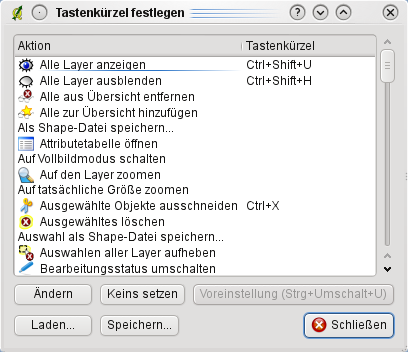
\includegraphics[clip=true, width=8cm]{shortcuts}
   \caption{Редактирование комбинаций клавиш \wincaption} \label{fig:shortcuts}
\end{figure}

Процесс редактирования комбинаций клавиш очень прост. Просто выберите
действие или инструмент из списка и нажмите на кнопке \button{Изменить},
\button{Удалить} или \button{По умолчанию}. Единожды определив свою
конфигурацию комбинаций клавиш, можно сохранить её в XML-файле и загрузить
на другом компьютере с установленной QGIS.

\subsection{Контекстная справка}\label{context_help}
\index{контекстная справка}

Если вам необходима помощь по конкретной теме, можно воспользоваться
контекстной справкой по нажатию кнопки \button{Справка}, доступной в
большинстве диалоговых окон, но, обратите внимание на то, что сторонние
модули могут перенаправлять на справочные материалы, размещенные в сети
Интернет.

\section{Рендеринг}\label{subsec:redraw_events}\index{рендеринг}

По умолчанию, QGIS перерисовывает все видимые слои всякий раз, когда
требуется обновление области карты. События, запускающие
процесс обновления карты, включают:

\begin{itemize}
\item Добавление слоя;
\item Панорамирование или масштабирование;
\item Изменение размеров окна QGIS;
\item Включение или отключение слоя/слоев в легенде.
\end{itemize}

В ряде случаев, QGIS позволяет контролировать процесс отрисовки.

\subsection{Видимость в пределах масштаба}\index{рендеринг!зависимый от масштаба}
\label{label_scaledepend}

Видимость слоя в пределах масштаба позволяет определить минимальный и
максимальный масштабы, при которых слой будет видимым. Для включения
видимости в пределах масштаба откройте диалоговое окно \dialog{Свойства},
дважды щёлкнув на слое в легенде. На вкладке \tab{Общие} нажмите флажок \\
\checkbox{Видимость в пределах масштаба} и установите значения минимального
и максимального масштаба.

Значения масштабов можно задать по первому масштабированию слоя, который
вы хотите использовать, отмечая значение масштаба в строке состояния QGIS.\index{масштаб}

\subsection{Управление отрисовкой карты}\label{label_controlmap}

Отрисовка карты может контролироваться одним из следующих способов:

\minisec{a) Приостановка отрисовки}\index{рендеринг!приостановка}
\label{label_suspendrender}

Для приостановки отрисовки карты снимите флажок \checkbox{Отрисовка}
в правом нижнем углу строки состояния. Когда флажок \checkbox{Отрисовка}
выключен, QGIS не будет перерисовывать карту в ответ на события,
описанные в разделе~\ref{subsec:redraw_events}. Приостановку отрисовки можно
использовать  в следующих случаях:

\begin{itemize}
\item Добавление нескольких слоев сразу и задание символики перед
нанесением на карту;
\item Добавление одного или нескольких больших слоев и включение видимости
в пределах масштаба перед нанесением на карту;
\item Добавление одного или нескольких больших слоев и масштабирование
к определенному виду перед нанесением на карту.
\end{itemize}

Включение флажка \checkbox{Отрисовка} активирует отрисовку и немедленно
обновляет содержимое карты.

\minisec{b) Добавление невидимых слоёв}\label{label_settinglayer}
\index{рендеринг!параметры}\index{слой!начальная видимость}

QGIS позволяет всегда загружать новые слои без отрисовки на карте. Это
означает, что слой будет добавлен к карте, но
флажок видимости в легенде изначально не будет активен. Для настройки
этого параметра выберите пункт меню \mainmenuopt{Установки} \arrow
\dropmenuopt{Параметры} и нажмите на вкладке \tab{Отрисовка}. Выключите
флажок \checkbox{Добавляемые на карту слои видимы по умолчанию}. Теперь
любой слой, добавленный к карте, по умолчанию будет невидимым (выключенным).

%\minisec{Stopping Rendering}\index{rendering!halting}
%\label{label_stoprender}
%
%To stop the map drawing, press the ESC key. This will halt the refresh of
%the map canvas and leave the map partially drawn. It may take a bit of time
%between pressing ESC and the time the map drawing is halted.
%
%\textbf{NOTE}: It is currently not possible to stop rendering - this was disabled
%in qt4 port because of User Interface (UI) problems and crashes.

\minisec{c) Обновление окна карты во время отрисовки}
\label{label_updatemap}\index{рендеринг!обновление при отрисовке}

Можно настроить параметр обновления карты во время прорисовки объектов.
По умолчанию, QGIS не отображает никаких объектов слоя на карте до тех пор,
пока не отрисуется весь слой. Для обновления окна карты в процессе загрузки данных,
выберите пункт меню \mainmenuopt{Установки} \arrow
\dropmenuopt{Параметры} и перейдите на вкладку \tab{Отрисовка}. Установите
число объектов в соответствующее значение для обновления карты во время
отрисовки. Установка значения равным 0 запрещает обновление карты во время
отрисовки слоя (значение по умолчанию). Установка слишком низкого значения
скажется на производительности"--- окно карты будет постоянно обновляться
во время загрузки данных. Приемлемыми значениями можно считать 500 и более объектов.

\minisec{d) Регулирование качества отрисовки}
\label{label_renderquality}\index{рендеринг!качество}

Для регулирования качества отрисовки карты можно задать два параметра.
Выберите пункт меню \mainmenuopt{Установки} \arrow \dropmenuopt{Параметры},
нажмите на вкладке \tab{Отрисовка} и включите или отключите следующие флажки.

\begin{itemize}
\item \checkbox{Рисовать сглаженные линии (снижает скорость отрисовки)}
\item \checkbox{Исправлять ошибки заливки полигонов}
\end{itemize}

\section{Измерения}\label{sec:measure}\index{измерения}

Измерения на карте работают только с Прямоугольными системами координат
(например, UTM). Если загруженная карта определена в географической
системе координат (широта/долгота), результаты измерений длин или площадей
будут неправильными. Чтобы этого избежать, необходимо указать
соответствующую систему координат (см. Раздел~\ref{label_projections}).
Оба измерительных инструмента также используют параметры прилипания, используемые
для оцифровки. Это может пригодиться, если необходимо провести измерения вдоль
линейных или площадных объектов в векторных слоях.

\subsection{Измерение длин, площадей и углов}
\index{измерения!длин}
\index{измерения!площадей}
\index{измерения!углов}

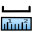
\includegraphics[width=0.7cm]{mActionMeasure}
QGIS позволяет измерить реальное расстояние между точками в
соответствии с заданным эллипсоидом. Для указания эллипсоида, выберите пункт
меню \mainmenuopt{Установки} \arrow \dropmenuopt{Параметры}, перейдите на вкладку
\tab{Инструменты} и выберите нужный вам эллипсоид. На этой же вкладке
можно выбрать цвет линии и единицы измерения по умолчанию (метры или футы).
Чтобы измерить расстояние, нажимайте на карте, ставя на ней точки. Длина
каждого сегмента получившейся линии, а также суммарный результат, будут
показаны в окне измерений. Прекратить измерение можно, щёлкнув правой кнопкой мыши.


\includegraphics[width=0.7cm]{mActionMeasureArea} Аналогично осуществляется измерение
площадей, в окне измерений выводится площадь указанной области.\\
Кроме того, инструмент измерений будет прилипать к объектам выбранного слоя,
при условии, что для слоя установлен порог прилипания
(см. раздел~\ref{snapping_tolerance}). Так, если необходимо провести точное
измерение длины линейного объекта или площади полигонального объекта, необходимо
настроить порог прилипания, а затем выбрать слой. Теперь, при использовании
инструмента измерений, при каждом нажатии кнопки мыши (в пределах порога
прилипания), курсор будет прилипать к объектам этого слоя. \\
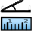
\includegraphics[width=0.7cm]{mActionMeasureAngle}
Также, вы можете измерять углы, выбрав инструмент Измерить угол. Курсор
станет крестообразным. Нажмите для создания первого сегмента угла, который
хотите измерить, затем перемещайте курсор для создания необходимого угла.
Результат измерения будет показан во всплывающем диалоговом окне.

\begin{figure}[ht]
\centering
   \subfloat[Измерение линий] {\label{subfig:measure_line}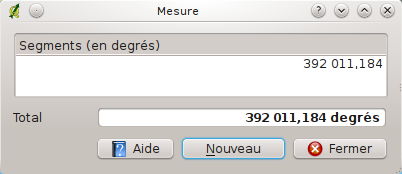
\includegraphics[clip=true, width=0.3\textwidth]{measure_line}}
     \hspace{0.33cm}
   \subfloat[Измерение площадей]{\label{subfig:measure_area}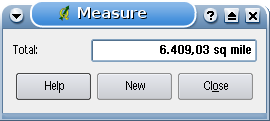
\includegraphics[clip=true, width=0.3\textwidth]{measure_area}}
     \hspace{0.33cm}
   \subfloat[Измерение углов]{\label{subfig:measure_angle}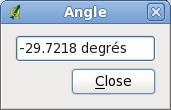
\includegraphics[clip=true, width=0.3\textwidth]{measure_angle}}
   \caption{Инструменты измерений \wincaption} \label{fig:measure}
\end{figure}


\section{Проекты}\label{sec:projects}\index{проекты}

Состояние сеанса в QGIS называется проектом. Настройки (установки) учитываются либо
для каждого проекта, либо как настройки по умолчанию для новых проектов
(см. Раздел~\ref{subsec:gui_options}). Сохранить состояние
вашего сеанса в файле проекта можно, используя пункт меню
\mainmenuopt{Файл} \arrow \dropmenuopttwo{mActionFileSave}{Сохранить проект}
или \mainmenuopt{Файл} \arrow
\dropmenuopttwo{mActionFileSaveAs}{Сохранить проект как\ldots}.

Загрузить сохраненный проект в QGIS можно, используя пункт меню
\mainmenuopt{Файл} \arrow \dropmenuopttwo{mActionFileOpen}{Открыть проект}
или \mainmenuopt{Файл} \arrow \dropmenuopt{Открыть недавние проекты}.

Если вы хотите очистить сеанс и начать новый, выберите \mainmenuopt{Файл}
\arrow \dropmenuopttwo{mActionFileNew}{Новый проект}. При выборе любого
из этих вариантов вам будет предложено сохранить существующий проект, если
были внесены изменения с момента его открытия или последнего сохранения.

Информация, сохраненная в файле проекта, включает в себя:

\begin{itemize}
\item Добавленные слои
\item Свойства слоёв, включая символику
\item Проекцию окна карты
\item Последний охват карты
\end{itemize}

Файл проекта сохраняется в формате XML, что делает возможным редактирование
его вручную. Формат файла проекта обновлялся (в сравнении с
предыдущими версиями QGIS) несколько раз. Файлы проектов ранних версий
QGIS больше не могут работать корректно. Чтобы включить предупреждение о том, что
используется файл проекта старого формата, активируйте следующие флажки на вкладке
\tab{Общие} пункта меню \mainmenuopt{Установки} \arrow \dropmenuopt{Параметры}: \\

\checkbox{Запрашивать сохранение изменений в проекте, когда это необходимо} \\
\checkbox{Предупреждать при попытке открытия файлов проекта старых версий QGIS}

\minisec{Свойства проекта}
В окне свойств проекта, находящегося в меню \nix{\mainmenuopt{Файл} \arrow
\dropmenuopt{Свойства проекта}} или \win{\mainmenuopt{Установки} \arrow
\dropmenuopt{Свойства проекта}}, настраиваются специальные параметры
проекта, включая:

\begin{itemize}
\item На вкладке \tab{Общие} определяется заглавие проекта, цвет выделения
и фона, единицы слоя, точность, и параметр сохранения относительных путей
к слоям. Также здесь настраиваются параметры топологического редактирования
и послойного прилипания.
\item Вкладка \tab{Система координат} позволяет выбрать систему координат
для данного проекта и включить преобразование координат векторных слоев
<<на лету>>, если используются слои с разными системами координат.
\item С помощью третьей вкладки \tab{Определяемые слои} можно настроить
(или отключить) то, какие слои будут реагировать на инструмент Определить
объекты. (cм. параграф <<Инструменты карты>> в Разделе~\ref{subsec:gui_options}
для включения <<Определения нескольких слоев>>.)
\end{itemize}

\section{Вывод}\label{sec:output}
\index{вывод!сохранить как изображение!компоновщик карты!быстрая печать}

Существует несколько способов для создания вывода из сеанса QGIS. Один из
них мы уже обсудили в Разделе~\ref{sec:projects}: это сохранение файла
проекта. Вот выборка других способов получения выходных файлов:

\begin{itemize}
\item Пункт меню \dropmenuopttwo{mActionSaveMapAsImage}{Сохранить как изображение\ldots}
открывает диалог сохранения файла, в котором можно выбрать название, путь сохранения
и формат изображения (PNG или JPG). Файл привязки с расширением PNGW
или JPGW, сохраняемый в ту же папку, обеспечивает географическую привязку
изображения.
\item Пункт меню \dropmenuopttwo{mActionFilePrint}{Создать компоновку карты}
открывает диалоговое окно, где можно создать макет и распечатать текущий
охват карты (см. Раздел~\ref{label_printcomposer}).
\item Модуль \toolbtntwo{quick_print}{Быстрая печать} позволяет напечатать
простую карту с минимальным количеством параметров (см. Раздел~\ref{quickprint}).
\end{itemize}

\section{Настройка QGIS}\label{subsec:gui_options}


\includegraphics[width=0.7cm,clip=true]{mActionOptions} Некоторые основные
параметры QGIS могут быть определены в диалоговом окне \dialog{Параметры}.
Выберите пункт меню \mainmenuopt{Установки} \arrow
\dropmenuopttwo{mActionOptions}{Параметры}. Параметры можно изменить на
следующих вкладках:

\minisec{Общие}

\begin{itemize}
\item \checkbox{Запрашивать сохранение изменений в проекте, когда это
необходимо}
\item \checkbox{Предупреждать при попытке открытия файлов проекта
старых версий QGIS}
\item Изменить цвет выделения и фона
\item Изменить тему значков (можно выбрать следующие варианты: default,
classic, gis и newgis)
\item \checkbox{Выводить имя слоя с заглавной буквы}
\item \checkbox{Показывать в легенде атрибуты классификации}
\item \checkbox{Создавать миниатюры в легенде для растровых слоев}
\item \checkbox{Не показывать заставку при запуске}
\item \checkbox{Открывать результаты определения во встраиваемом окне
(требуется перезапуск QGIS)}
\item \checkbox{Открывать таблицу атрибутов во встраиваемом окне}
\item \checkbox{Добавлять слои PostGIS двойным щелчком и включить
расширенную выборку}
\item \checkbox{Добавлять новые слои в активную группу}
\item Вид таблицы атрибутов (можно выбрать следующие варианты: Показывать
все объекты (по умолчанию); Показывать выделенные объекты; Показывать
объекты, видимые в области карты).
\end{itemize}

\minisec{Отрисовка}

\begin{itemize}
\item \checkbox{Добавляемые на карту слои видимы по умолчанию}
\item Количество объектов для отрисовки между обновлениями экрана.
\item \checkbox{Использовать кэш для ускорения перерисовки там,
где это возможно}
\item \checkbox{Рисовать сглаженные линии (снижает скорость отрисовки)}
\item \checkbox{Исправлять ошибки заливки полигонов}
\item \checkbox{Использовать новую реализацию отрисовки условных знаков}
\item Добавить/Удалить пути поиска значков в формате SVG (Scalable Vector Graphics)
\end{itemize}

Дополнительно, на вкладке \tab{Общие} меню \mainmenuopt{Установки} \arrow
\dropmenuopttwo{mActionOptions}{Свойства проекта} можно задать, какие пути
сохранения использовать для текстур SVG,"--- абсолютные или относительные.

\minisec{Инструменты}

\begin{itemize}
\item Режим определения используется для указания того, какие слои будут
показываться при использовании инструмента Определить объекты. При выборе
\usertext{Сверху вниз} или \usertext{Сверху вниз, до первого найденного}
вместо \usertext{Текущий слой}, при использовании инструмента Определить
объекты будут показаны атрибуты всех определяемых слоев (см. Раздел~\ref{sec:projects}
<<Свойства проекта>> для настройки определяемых слоев).
\item \checkbox{Открывать форму, если найден один объект}
\item Установить радиус поиска для определения объектов и всплывающих
описаний (задается в процентах от ширины видимой карты)
\item Установить эллипсоид для вычисления расстояний
\item Установить цвет линии для инструментов измерений
\item \radiobuttonon{{}Установить единицы измерения по умолчанию (метры
или футы)}
\item \radiobuttonon{{}Установить единицы измерения углов (градусы,
радианы или грады)}
\item Установить действие при прокрутке колеса мыши (Увеличить, Увеличить
и центрировать, Увеличить в положении курсора, Ничего)
\item Установить фактор увеличения для колеса мыши
\end{itemize}

\minisec{Совмещение}

\begin{itemize}
\item Установить алгоритм размещения для подписей (выберите вариант: central
point (по умолчанию), chain, popmusic tabu chain, popmusic tabu и
popmusic chain)
\end{itemize}

\minisec{Оцифровка}

\begin{itemize}
\item Установить цвет и толщину линии
\item Установить режим прилипания по умолчанию (к вершинам, к сегментам,
к вершинам и сегментам)
\item Установить порог прилипания по умолчанию (в единицах карты или
пикселях)
\item Установить радиус поиска для редактирования вершин (в единицах
карты или пикселях)
\item \checkbox{Показывать маркеры только для выбранных объектов}
\item Установить стиль маркера (перекрестие (по умолчанию), полупрозрачный
круг или без маркера) и размер маркера
\item \checkbox{Не показывать всплывающее окно ввода атрибутов для каждого
создаваемого объекта}
\end{itemize}

\minisec{Система координат}

\begin{itemize}
\item \radiobuttonoff{{}Запрашивать систему координат}
\item \radiobuttonoff{{}Использовать значение по умолчанию для данного
проекта}
\item \radiobuttonon{{}Использовать нижеприведенную глобальную систему
координат}
\item Выбрать глобальную систему координат\ldots
\end{itemize}

\minisec{Язык}

\begin{itemize}
\item \checkbox{Переопределить системный язык и использовать вместо системного}
\item Дополнительная информация о системном языке
\end{itemize}

\minisec{Сетевые соединения}

\begin{itemize}
\item \checkbox{Таймаут для сетевых запросов (мс)}
\item \checkbox{Использовать прокси-сервер для внешних соединений} и
настроить поля Узел, Порт, Пользователь, и Пароль.
\item Установить \dropmenuopt{Тип прокси}
 \begin{itemize}
  \item \dropmenuopt{Default Proxy}: Прокси определяется настройками
  приложения
  \item \dropmenuopt{Socks5Proxy}: Общий прокси для любого вида связи.
  Поддерживаются TCP, UDP, привязка к порту (входящие соединения) и
  авторизация.
  \item \dropmenuopt{HttpProxy}: Реализован с использованием комманды
  <<СONNECT>>, поддерживает только исходящие TCP соединения; поддерживает
  авторизацию.
  \item \dropmenuopt{HttpCachingProxy}: Использует стандартные команды
  HTTP, имеет смысл использовать только с запросами HTTP
  \item \dropmenuopt{FtpCachingProxy}: Реализован посредством FTP прокси,
  имеет смысл использовать только с запросами FTP
 \end{itemize}
\end{itemize}

Если вы не хотите использовать прокси-сервер для некоторых адресов, можно
добавить их в текстовое поле ниже (см. Рисунок~\ref{fig:proxy-settings}),
нажав кнопку \button{Добавить}. После двойного нажатия на только что
созданной строке адреса URL (Uniform Resource Locator), введите адрес,
для которого не хотите использовать прокси-сервер. Нажатие на кнопке
\button{Удалить} удаляет выбранную строку адреса.

Для получения более детальной информации о различных настройках прокси-сервера,
обратитесь к Руководству QT-library-documentation по адресу \\
\url{http://doc.trolltech.com/4.5/qnetworkproxy.html#ProxyType-enum}.

\begin{figure}[ht]
   \centering
   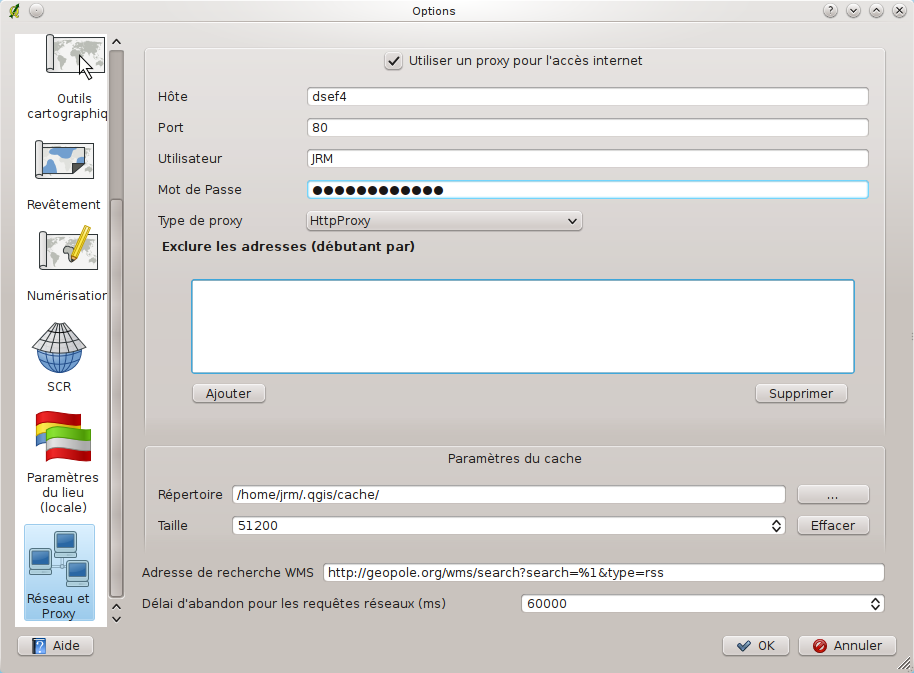
\includegraphics[clip=true, width=14cm]{proxy-settings}
   \caption{Настройка прокси в \qg \wincaption}
   \label{fig:proxy-settings}
\end{figure}

\begin{Tip} \caption{\textsc{Использование прокси-серверов}}
Использование прокси-серверов иногда может быть довольно сложным. Для
проверки вышеописанных типов прокси, действуйте методом <<проб и ошибок>>,
проверяя в каждом случае успешность соединений.
\end{Tip}

Можно настроить параметры в соответствии с вашими потребностями. Внесение
некоторых изменений может потребовать перезапуска QGIS для их применения.

\begin{itemize}
\item \nix{параметры сохраняются в текстовом файле: \$HOME/.config/QuantumGIS/qgis.conf}
\item \osx{ваши настройки можно найти в файле: \$HOME/Library/Preferences/org.qgis.qgis.plist}
\item \win{параметры хранятся в ветке системного реестра:}
\begin{verbatim}
\\HKEY\CURRENT\USER\Software\QuantumGIS\qgis
\end{verbatim}
\end{itemize}

\section{Инструменты аннотации}\label{sec:annotations}
\index{аннотации}
\index{текстовые аннотации|see{аннотации}}

Инструмент 
\includegraphics[width=0.7cm,clip=true]{mActionTextAnnotation}
Текстовая аннотация на панели атрибутов предоставляет возможность размещения
форматированного текста в выноске на карте QGIS. Выберите инструмент аннотаций
и нажмите внутри окна карты.

\begin{figure}[ht]
   \centering
   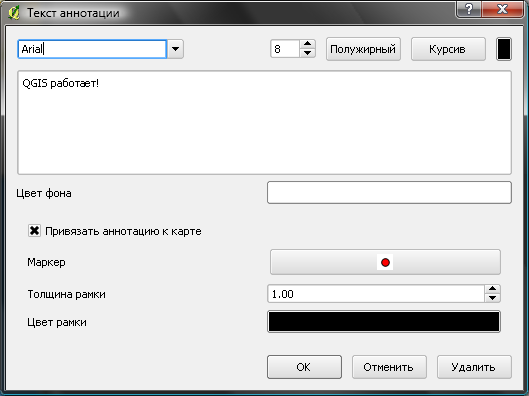
\includegraphics[clip=true, width=12cm]{annotation}
   \caption{Диалоговое окно текста аннотации \wincaption}
   \label{fig:annotation}
\end{figure}

Двойное нажатие на сноске открывает диалоговое окно с различными параметрами.
Здесь находится текстовый редактор для ввода форматированного текста и прочие
настраиваемые параметры. Например, можно привязать аннотацию к карте
(обозначив маркером) или располагать ее свободно относительно карты. Аннотацию
можно перемещать относительно карты (перетаскиванием маркера) или перемещать
саму сноску.

Инструмент Переместить аннотацию

\includegraphics[width=0.7cm,clip=true]{mActionAnnotation} позволяет
перемещать аннотацию в окне карты.

\minisec{Диалоговая аннотация}\index{аннотации}
\index{диалоговые аннотации|see{аннотации}}

Дополнительно, вы можете создавать свои собственные диалоговые аннотации.
Инструмент Диалоговая аннотация

\includegraphics[width=0.7cm,clip=true]{mActionFormAnnotation} полезен
для отображения атрибутов векторного слоя в виде индивидуальной формы,
настроенной в Qt~Designer (см. Рисунок~\ref{fig:custom-annotations}).
Это похоже на конструктор форм для инструмента Определить объекты, но
отображается в виде аннотации. Для получения дополнительной информации
посетите блог QGIS \url{http://blog.qgis.org/node/143}.

\begin{figure}[ht]
   \centering
   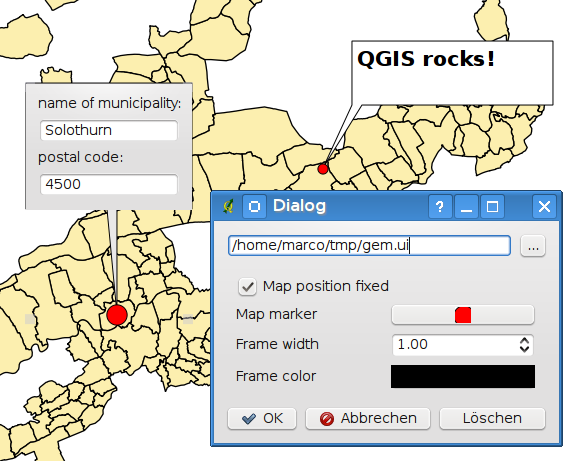
\includegraphics[clip=true, width=10cm]{custom_annotation}
   \caption{Настраиваемая диалоговая аннотация \wincaption}
   \label{fig:custom-annotations}
\end{figure}

\newpage

\section{Пространственные закладки}\label{sec:bookmarks}
\index{закладки}
\index{пространственные закладки|see{закладки}}

Пространственные закладки позволяют создавать своеобразные <<закладки>>
географического положения и возвращаться к ним позднее.

\subsection{Создание закладки}
Для создания закладки:
\begin{enumerate}
\item Масштабируйте или панорамируйте карту до интересующей вас территории.
\item Выберите пункт меню \mainmenuopt{Вид} \arrow
\dropmenuopt{Новая закладка} или нажмите \keystroke{Ctrl-B}.
\item Введите описательное имя для закладки (до 255 символов).
\item Нажмите \button{OK}, чтобы добавить закладку, или \button{Отменить}
для выхода без добавления закладки.
\end{enumerate}

Помните, что можно иметь множество закладок с одинаковыми названиями.

\subsection{Работа с закладками}
Для использования закладок и управления ими выберите пункт меню
\mainmenuopt{Вид} \arrow \\ \dropmenuopt{Показать закладки}. Диалоговое
окно \dialog{Пространственные закладки} позволяет просматривать или удалять
закладки. Но нельзя редактировать название закладки или координаты.

\subsection{Просмотр закладки}
В диалоговом окне \dialog{Пространственные закладки}, выберите необходимую
закладку, нажав на неё, затем нажмите кнопку \button{Увеличить до}. Также
можно просмотреть закладку, дважды нажав на неё.

\subsection{Удаление закладки}
Для удаления закладки из диалогового окна \dialog{Пространственные закладки}
выберите е~ и нажмите кнопку \button{Удалить}. Подтвердите ваш выбор
нажатием на кнопке \button{ОК} или отмените удаление нажатием кнопки
\button{Отменить}.

\section{GPS-слежение}\label{sec:gpstracking}

Для включения GPS-слежения в QGIS необходимо выбрать \mainmenuopt{Вид}
\arrow \dropmenuopt{GPS-слежение}. Появится новое окно, пристыкованное
с левой стороны рабочей области.

Существует 4~варианта окна GPS-слежения (см. Рисунок~\ref{fig:gpstrack_live}).

\begin{description}
 \item[(a)] 
\includegraphics[width=0.5cm,clip=true]{mActionToggleEditing}
 Координаты текущего местоположения и кнопки добавления вершин и объектов
 \item[(b)] 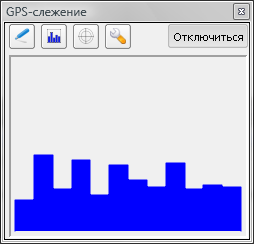
\includegraphics[width=0.5cm,clip=true]{gpstrack_barchart}
 Мощность сигнала присоединенных спутников GPS
 \item[(c)] 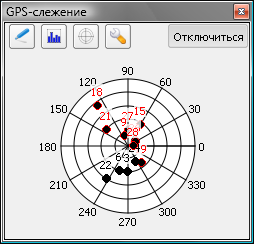
\includegraphics[width=0.5cm,clip=true]{gpstrack_polarchart}
 Экран положения спутников GPS, отображающий количество и расположение спутников
 \item[(d)] 
\includegraphics[width=0.5cm,clip=true]{mActionOptions}
 Экран параметров GPS (см. Рисунок \ref{fig:gpstrack_options}).
\end{description}

При подключенном GPS-приемнике (должен поддерживаться вашей операционной
системой), простое нажатие на кнопке \button{Подключиться} подключает
GPS к QGIS. Второе нажатие на кнопке (теперь уже \button{Отключиться})
отключает GPS-приемник от компьютера.

[ ВАЖНО ]: Если вы хотите записать текущее местоположение или путь,
необходимо сначала создать новый векторный слой и переключиться в режим
редактирования.

\begin{figure}[ht]
\centering
   \subfloat[Координаты текущего местоположения] {\label{subfig:gpstrack_main}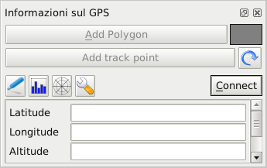
\includegraphics[clip=true, width=0.3\textwidth]{gpstrack_main}}
     \hspace{0.33cm}
   \subfloat[Мощность сигнала GPS]{\label{subfig:gpstrack_stren}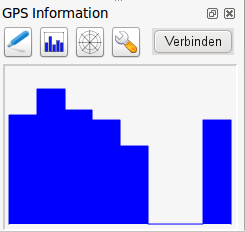
\includegraphics[clip=true, width=0.3\textwidth]{gpstrack_stren}}
     \hspace{0.33cm}
   \subfloat[Положение спутников GPS]{\label{subfig:gpstrack_polar}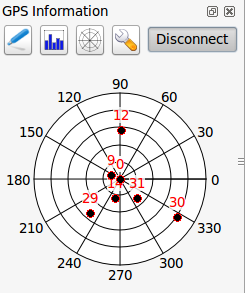
\includegraphics[clip=true, width=0.3\textwidth]{gpstrack_polar}} \\
\caption{Варианты окна GPS-слежения \nixcaption} \label{fig:gpstrack_live}
\end{figure}

\subsection{Координаты текущего местоположения}

\includegraphics[width=0.5cm,clip=true]{mActionToggleEditing} Если GPS-приемник
получает сигнал со спутников, вы увидите ваше текущее положение в формате широты
и долготы, а также высоту над уровнем моря, как показано на
Рисунке~\ref{subfig:gpstrack_main}

\subsection{Мощность сигнала GPS}
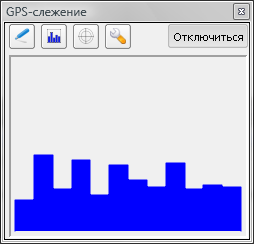
\includegraphics[width=0.5cm,clip=true]{gpstrack_barchart} Здесь можно
видеть мощность сигнала спутников, с которых вы получаете сигнал
(Рисунок~\ref{subfig:gpstrack_stren}).

\subsection{Положение спутников GPS}
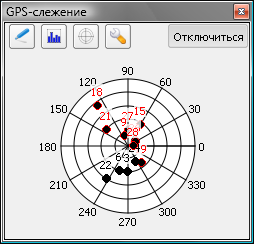
\includegraphics[width=0.5cm,clip=true]{gpstrack_polarchart} Если вы
хотите знать, где на небесной сфере располагаются все присоединенные спутники,
переключитесь на окно Положение спутников
(Рисунок~\ref{subfig:gpstrack_polar}). Также здесь можно увидеть
идентификационные номера (ID) спутников, с которых вы получаете сигнал.

\subsection{Параметры GPS}

\includegraphics[width=0.5cm,clip=true]{mActionOptions} В случае
возникновения проблем с соединением, можно переключиться с
\radiobuttonon{{}Автоопределение} на
\radiobuttonon{{}Использовать указанный путь}, и выбрать путь (и порт)
присоединенного GPS-приемника. Нажатие кнопки \button{Подключиться}
снова инициирует соединение с GPS-приемником.

Ползунком \slider{Размер курсора} можно уменьшать и увеличивать курсор
текущего местоположения в окне карты. Включение параметра
\radiobuttonon{{}Автоматически создавать вершины} в Оцифровке будет
автоматически записывать трек в активный векторный слой (разумеется,
слой должен быть в режиме редактирования).

Установка параметра центрирования карты позволяет контролировать, в каких
случаях будет обновляться окно карты: в случае, если записываемые
координаты выходят за текущий охват карты, либо всегда (или же никогда).

Параметр <<Цвет трека>> задает цвет и толщину отрисовываемого трека.

Если вы хотите добавлять объекты вручную, вернитесь обратно к окну

\includegraphics[width=0.5cm,clip=true]{mActionToggleEditing} <<Координаты
текущего местоположения>> и нажмите \button{Добавить объект}. Также, если
не активна функция <<Автоматически создавать вершины>>, и вы хотите создавать
вершины вручную, нажмите \button{Добавить вершину}

\begin{figure}[ht]
   \centering
   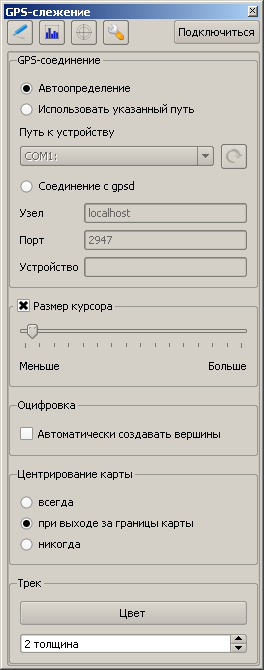
\includegraphics[clip=true, width=5cm]{gpstrack_options}
   \caption{Окно параметров GPS-слежения \wincaption}
   \label{fig:gpstrack_options}
\end{figure}

\FloatBarrier
